% Mestre em LaTeX - v0.2
% Copyleft 2008-2010 Bruno C. Vellutini - http://organelas.com/
%
% Permission is hereby granted, free of charge, to any person obtaining a copy
% of this software and associated documentation files (the "Software"), to deal
% in the Software without restriction, including without limitation the rights
% to use, copy, modify, merge, publish, distribute, sublicense, and/or sell
% copies of the Software, and to permit persons to whom the Software is
% furnished to do so, subject to the following conditions:
%
% THE SOFTWARE IS PROVIDED "AS IS", WITHOUT WARRANTY OF ANY KIND, EXPRESS OR
% IMPLIED, INCLUDING BUT NOT LIMITED TO THE WARRANTIES OF MERCHANTABILITY,
% FITNESS FOR A PARTICULAR PURPOSE AND NONINFRINGEMENT. IN NO EVENT SHALL THE
% AUTHORS OR COPYRIGHT HOLDERS BE LIABLE FOR ANY CLAIM, DAMAGES OR OTHER
% LIABILITY, WHETHER IN AN ACTION OF CONTRACT, TORT OR OTHERWISE, ARISING FROM,
% OUT OF OR IN CONNECTION WITH THE SOFTWARE OR THE USE OR OTHER DEALINGS IN
% THE SOFTWARE.
%
% Ou seja utilize e modifique os arquivos como desejar.
% 
% Para mais informações visite http://code.google.com/p/mestre-em-latex/

% Classe do documento
\documentclass[twoside,a4paper,12pt]{report}


% Pacotes e comandos customizados
%%% Pacotes utilizados %%%

%% Codificação e formatação básica do LaTeX
% Suporte para português (hifenação e caracteres especiais)
\usepackage[english,brazilian]{babel}

% Codificação do arquivo
\usepackage[utf8]{inputenc}

% Mapear caracteres especiais no PDF
\usepackage{cmap}

% Codificação da fonte
%\usepackage[T1]{fontenc}
\usepackage{times}


% Essencial para colocar funções e outros símbolos matemáticos
\usepackage{amsmath,amssymb,amsfonts,textcomp}

%% Layout
% Customização do layout da página, margens espelhadas
\usepackage[twoside]{geometry}
% Aumenta as margens internas para espiral
\geometry{bindingoffset=10pt}
% Só pra ajustar o layout
\setlength{\marginparwidth}{90pt}
%\usepackage{layout}

% Para definir espaçamento entre as linhas
\usepackage{setspace}

% Espaçamento do texto para o frame
\setlength{\fboxsep}{1em}

% Faz com que as margens tenham o mesmo tamanho horizontalmente
%\geometry{hcentering}

%% Elementos Gráficos
% Para incluir figuras (pacote extendido)
\usepackage[]{graphicx}

% Suporte a cores
\usepackage{color}

% Criar figura dividida em subfiguras
\usepackage{subfig}
\captionsetup[subfigure]{style=default, margin=0pt, parskip=0pt, hangindent=0pt, indention=0pt, singlelinecheck=true, labelformat=parens, labelsep=space}

% Caso queira guardar as figuras em uma pasta separada
% (descomente e) defina o caminho para o diretório:
\graphicspath{{./Figuras/}}

% Customizar as legendas de figuras e tabelas
\usepackage{caption}

% Criar ambientes com 2 ou mais colunas
\usepackage{multicol}

% Ative o comando abaixo se quiser colocar figuras de fundo (e.g., capa)
%\usepackage{wallpaper}
% Exemplo para inserir a figura na capa está no arquivo pre.tex (linha 7)
% Ajuste da posição da figura no eixo Y
%\addtolength{\wpYoffset}{-140pt}
% Ajuste da posição da figura no eixo X
%\addtolength{\wpXoffset}{36pt}

%% Tabelas
% Elementos extras para formatação de tabelas
\usepackage{array}

% Tabelas com qualidade de publicação
\usepackage{booktabs}

% Para criar tabelas maiores que uma página
\usepackage{longtable}

% adicionar tabelas e figuras como landscape
\usepackage{lscape}

%% Lista de Abreviações
% Cria lista de abreviações
\usepackage[notintoc,portuguese]{nomencl}
\makenomenclature



\usepackage{cite}


%% Notas de rodapé
% Lidar com notas de rodapé em diversas situações
\usepackage{footnote}

% Notas criadas nas tabelas ficam no fim das tabelas
\makesavenoteenv{tabular}

%% Links dinâmicos
% Suporte para hipertexto, links para referências e figuras
\usepackage{hyperref}
% Configurações dos links e metatags do PDF a ser gerado
\hypersetup{colorlinks=true, linkcolor=blue, citecolor=blue, filecolor=blue, pagecolor=blue, urlcolor=green,
            pdfauthor={Nome do Autor},
            pdftitle={Título do Projeto},
            pdfsubject={Assunto do Projeto},
            pdfkeywords={palavra-chave, palavra-chave, palavra-chave},
            pdfproducer={Latex},
            pdfcreator={pdflatex}}

% Conta o número de páginas
\usepackage{lastpage}

%% Referências bibliográficas e afins
% Formatar as citações no texto e a lista de referências
\usepackage{natbib}

% Adicionar bibliografia, índice e conteúdo na Tabela de conteúdo
% Não inclui lista de tabelas e figuras no índice
\usepackage[nottoc,notlof,notlot]{tocbibind}

%% Pontuação e unidades
% Posicionar inteligentemente a vírgula como separador decimal
\usepackage{icomma}

% Formatar as unidades com as distâncias corretas
\usepackage[tight]{units}

%algoritmos
\usepackage{algorithm}
\usepackage{algorithmic}
\usepackage{lipsum}


%% Cabeçalho e rodapé
% Controlar os cabeçalhos e rodapés
\usepackage{fancyhdr}
% Usar os estilos do pacote fancyhdr
\pagestyle{fancy}
\fancypagestyle{plain}{\fancyhf{}}
% Limpar os campos do cabeçalho atual
\fancyhead{}
% Número da página do lado esquerdo [L] nas páginas ímpares [O] e do lado direito [R] nas páginas pares [E]
\fancyhead[LO,RE]{\thepage}
% Nome da seção do lado direito em páginas ímpares
\fancyhead[RO]{\nouppercase{\rightmark}}
% Nome do capítulo do lado esquerdo em páginas pares
\fancyhead[LE]{\nouppercase{\leftmark}}
% Limpar os campos do rodapé
\fancyfoot{}
% Omitir linha de separação entre cabeçalho e conteúdo
\renewcommand{\headrulewidth}{0pt}
% Omitir linha de separação entre rodapé e conteúdo
\renewcommand{\footrulewidth}{0pt}
% Altura do cabeçalho
\headheight 13.6pt

%% Inserir comentários no texto
% Marcar mudanças e fazer comentários
%\usepackage[margins]{trackchanges}
% Iniciais do autor
%\renewcommand{\initialsTwo}{bcv}
% Notas na margem interna
%\reversemarginpar

%% Comandos customizados

% Espécie e abreviação
\newcommand{\subde}{\emph{Clypeaster subdepressus}}
\newcommand{\subsus}{\emph{C.~subdepressus}}

% Título do projeto
\newcommand{\titulo}{Título original do projeto}
\newcommand{\nomedoaluno}{Nome Completo do Aluno}


\renewcommand\citeleft{(}
\renewcommand\citeright{)}

%% Pacotes não implementados
% Para não sobrar espaços em branco estranhos
%\widowpenalty=1000
%\clubpenalty=1000

\usepackage{times}
%\usepackage[brazil]{babel}
%\usepackage{listings}
\usepackage{graphicx}
\usepackage{epstopdf}

\usepackage[utf8]{inputenc}
%\usepackage{color}
%\usepackage{colortbl}

% Início do texto
\begin{document}

% Capa
\begin{titlepage}
% Se quiser uma figura de fundo na capa ative o pacote wallpaper
% e descomente a linha abaixo.
% \ThisCenterWallPaper{0.8}{nomedafigura}

\begin{center}
{\LARGE Luis Felipe Sant'Ana}
\par
\vspace{200pt}
{\Huge  Balanceamento de Carga Dinâmico em Aglomerados de GPUs }
\par
\vfill
\textbf{{\large Santo André}\\
{\large 2014}}
\end{center}
\end{titlepage}

% A partir daqui páginas sem cabeçalho
\pagestyle{empty}
% Faz com que a página seguinte sempre seja ímpar (insere pg em branco)
\cleardoublepage

% Números das páginas em algarismos romanos
\pagenumbering{roman}

% Página de Rosto
\begin{center}
{\LARGE Luis Felipe Sant'Ana}
\par
\vspace{200pt}
{\Huge  Balanceamento de Carga Dinâmico em Aglomerados de GPUs}
\end{center}
\par
\vspace{90pt}
\hspace*{175pt}\parbox{7.8cm}{{\large Dissertação Apresentada ao Centro de Matemática, Computação e 
Cognição da Universidade Federal do ABC, para a obtenção do Título de Mestre em Ciência da Computação.}}

\par
\vspace{1em}
\hspace*{175pt}\parbox{7.6cm}{{\large Orientador: Dr. Raphael Y. de Camargo}}

\par
\vfill
\begin{center}
\textbf{{\large Santo André}\\
{\large 2014}}
\end{center}

\newpage

% Ficha Catalográfica
\hspace{8em}\fbox{\begin{minipage}{11cm}
Sant Ana, Luis F.

\hspace{2em} Balanceamento de Carga Dinâmico em Aglomerados de GPUs

\hspace{2em}10 páginas

\hspace{2em}Dissertação de Mestrado - Centro de Matemática, Computação e Cognição da Universidade Federal do ABC.

\begin{enumerate}
\item Programação Paralela 
\item Balanceamento de Carga
\item GPGPU
\end{enumerate}
I. Universidade Federal do ABC. Centro de Matemática, Computação e Cognição.

\end{minipage}}
\par
\vspace{2em}
\begin{center}
{\LARGE\textbf{Comissão Julgadora:}}

\par
\vspace{8em}
\begin{tabular*}{\textwidth}{@{\extracolsep{\fill}}l l}
\rule{16em}{1px} 	& \rule{15em}{1px} \\
Prof. Dr. 		& Prof. Dr. \\
XX		&  YY
\end{tabular*}

\par
\vspace{10em}
\parbox{16em}{\rule{16em}{1px} \\
Prof. Dr. \\
Raphael Yokoingawa de Camargo}
\end{center}

%%\newpage

% Dedicatória
% Posição do texto na página
%%\vspace*{0.75\textheight}
%%\begin{flushright}
%%  \emph{Dedico este trabalho a todos aqueles que me ajudaram na busca do conhecimento.}
%%\end{flushright}

%\newpage

% Epígrafe
%%\vspace*{0.4\textheight}
%%\noindent{\LARGE\textbf{Bonito}}
% Tudo que você escreve no verbatim é renderizado literalmente (comandos não são interpretados e os espaços são respeitados)
%%\begin{verbatim}
%%O que é bonito?
%%É o que persegue o infinito;
%%Mas eu não sou
%%Eu não sou, não…
%%Eu gosto é do inacabado,
%%O imperfeito, o estragado, o que dançou
%O que dançou…
%Eu quero mais erosão
%Menos granito.
%Namorar o zero e o não,
%Escrever tudo o que desprezo
%E desprezar tudo o que acredito.
%Eu não quero a gravação, não,
%Eu quero o grito.
%Que a gente vai, a gente vai
%E fica a obra,
%Mas eu persigo o que falta
%Não o que sobra.
%%%%Eu quero tudo que dá e passa.
%Quero tudo que se despe,
%Se despede, e despedaça.
%O que é bonito…
%%\end{verbatim}
%%\begin{flushright}
%%Lenine e Bráulio Tavares
%%\end{flushright}

\newpage

% Agradecimentos

% Espaçamento duplo
%\begin{doublespacing}

%\noindent{\LARGE\textbf{Agradecimentos}}

%Agradeço ao meu orientador, amigos de curso e todos aqueles que contribuiram de alguma %forma à minha formação. 

%\end{doublespacing}
%\newpage

\vspace*{10pt}
% Abstract
\begin{center}
  \emph{\begin{large}Resumo\end{large}}\label{resumo}
\vspace{2pt}
\end{center}
% Pode parecer estranho, mas colocar uma frase por linha ajuda a organizar e reescrever o texto quando necessário.
% Além disso, ajuda se você estiver comparando versões diferentes do mesmo texto.
% Para separar parágrafos utilize uma linha em branco.
\noindent

\begin{doublespacing}
O uso de GPUs em aplicações científicas está cada vez mais difundido, com
aplicações em áreas como física, química e bioinformática. Mesmo com o ganho de
desempenho obtido com o uso de uma GPU, algumas aplicações ainda requerem
elevados tempos de execução. Para esses problemas a utilização de
\textit{clusters} de GPUs surgem como uma possível solução. Mas é comum termos
máquinas contendo GPUs com variadas capacidades e de diferentes gerações,
resultando em \textit{clusters} heterogêneos. Neste cenário, um dos pontos fundamentais é
o balanceamento de carga entre as diferentes GPUs, com o objetivo de maximizar a
utilização das GPUs e/ou minimizar o tempo de execução da aplicação. Este
projeto tem como objetivo o desenvolvimento de um algoritmo de balanceamento de
cargas dinâmico entre GPUs heterogêneas. Implementaremos o algoritmo em uma
biblioteca existente que facilita o desenvolvimento de aplicações para
aglomerados de GPUs e compararemos seu desempenho com outros algoritmos de
balanceamento de carga.

\end{doublespacing}

\par
\vspace{1em}
\noindent\textbf{Palavras-chave:} Programação Paralela, Balanceamento de Carga, GPGPU.
\newpage

% Criei a página do abstract na mão, por isso tem bem mais comandos do que o resumo acima, apesar de serem idênticas.
\vspace*{10pt}
% Abstract
\begin{center}
  \emph{\begin{large}Abstract\end{large}}\label{abstract}
\vspace{2pt}
\end{center}

% Selecionar a linguagem acerta os padrões de hifenação diferentes entre inglês e português.
\selectlanguage{english}

\begin{doublespacing}

\noindent
The use of GPUs for scientific applications is becoming more widespread, with applications in fields such as physics, chemistry and bioinformatics. Even with the performance gain obtained by using a GPU, some applications require even higher execution times. For these problems the use of GPU clusters arise as a possible solution. But it is common to machines containing GPUs with different capabilities and different generations, resulting in heterogeneous clusters. In this scenario, one of the key points is the load balancing between different GPUs, with the goal of maximizing the use of GPUs and / or minimize the execution time of the application. This project aims to develop an algorithm for dynamic load balancing among heterogeneous GPUs. We implement the algorithm in an existing library that facilitates the development of applications for clusters of GPUs and compare their performance with other load balancing algorithms.

\end{doublespacing}

\par
\vspace{1em}
\noindent\textbf{Keywords:} Parallel Programming, Load Balancing, CUDA, GPGPU. 

% Voltando ao português...

\selectlanguage{brazilian}

%\newpage

% Lista de figuras
\listoffigures

% Lista de tabelas
\listoftables

% Abreviações
% Para imprimir as abreviações siga as instruções em 
% http://code.google.com/p/mestre-em-latex/wiki/ListaDeAbreviaturas
\printnomenclature

% Índice
\tableofcontents
   % Capa, prefácio e afins
%% Faz com que o ínicio do capítulo sempre seja uma página ímpar
%\cleardoublepage
% Inclui o cabeçalho definido no meta.tex
\pagestyle{fancy}

% Números das páginas em arábicos
\pagenumbering{arabic}

\chapter{Introdução}\label{intro}

\section{Escalonamento}

Escalonamento é um processo de tomada de decisão que é usado como base em muitas insdústrias manufatureiras e serviços industriais. Ele lida com a alocação de recursos para tarefas a fim de fornecer períodos de tempo a cada tarefa  e o fim é otimizar um ou mais objetivos.

Encontrar um escalonamento significa encontrar, para cada tarefa, uma alocação de um ou mais intervalos de tempo, em uma ou mais máquinas. O problema de escalonamento correspondente é encontrar um escalonamento que satisfaça um determinado conjunto de restrições.

Em um ambiente genérico de fabricação, o papel do escalonamento das tarefas é 
destacado nas ordens de serviço que são lançadas na configuração da fabricação,
em forma de tarefas com datas de entrega associadas. Essas tarefas 
frequentemente devem ser processadas em máquinas em uma dada ordem ou 
sequência. Os processamentos das tarefas podem atrasar, se certas máquinas 
estiverem ocupadas. Eventos imprevistos no chão-de-fábrica, tais como quebra de 
máquinas ou tempos de processamento maiores que os previstos, também devem 
ser levados em consideração, desde que esses eventos venham a impactar 
diretamente o escalonamento das tarefas. Neste ambiente, o desenvolvimento de um escalonador de tarefas detalhado ajuda a manter a eficiência e o controle das 
operações. 

O chão-de-fábrica não é a única parte da organização que impacta o 
processo de escalonamento. O escalonador também é afetado pelo processo de 
planejamento da produção que lida com o planejamento a médio e a longo prazos 
para toda a organização. Esse processo tenta otimizar toda linha de produtos da 
empresa e a alocação de recursos baseados em seus níveis de estoque, previsões 
de demanda e necessidades de recursos. As decisões tomadas neste nível mais alto 
de planejamento podem impactar o processo de escalonamento diretamente. 

Um exemplo de escalonamento é na indústria de semicondutores  no qual o objetivo é maximizar o tempo de utilização dos equipamentos e minimizar o tempo ocioso e de configuração dos mesmos.

\subsection{Notação dos problemas de escalonamento}
Associados às tarefas, existem as seguintes informações:
\begin{itemize}
\item Tempo de execução ($p_{ij}$) tempo necessário para a execução da tarefa $t_i$ na máquina $m_j$. Denotado apenas por $p_i$ se todas as máquinas forem idênticas
\item Data de disponibilidade ($r_i$) instante em que a tarefa $t_i$ se torna disponível para ser executada
\item Prazo ($d_i$) instante de tempo no qual a tarefa $t_i$ deve estar pronta
\item Peso ($w_i$) normalmente indica um fator de prioridade da tarefa $t_i$
\end{itemize}

A notação utilizada para representar os problemas de escalonamento, é representada pela tripla:   

$\alpha | \beta | \gamma$

$\alpha$ 	que descreve os recursos disponíveis

$\beta$ que descreve as tarefas a serem executadas

$\gamma$ que descreve o critério de otimização

$\alpha$ pode ser representado por:

\begin{itemize}
\item 1 uma única máquina
\item $P$ ou $P_m$ m máquinas paralelas idênticas cada tarefa $t_i$ pode ser processada em qualquer uma das $m$ máquinas por $p_i$ unidades de tempo, se uma tarefa só puder ser executada em um subconjunto das máquinas, a restrição será indicada no campo 
\item $P \infty$ ou $\overline{P}$ é o número ilimitado de máquinas idênticas
\end{itemize}

$\beta$ pode ser representado por:
\begin{itemize}
\item $Q_m$ máquinas paralelas uniformes no qual $m$ máquinas  operam com 
velocidades iguais (a máquina $m_j$ opera com velocidade $v_j$) $p_{ij} = p_i=v_j$
\item $R_m$ máquinas paralelas não-relacionadas, $m$ máquinas diferentes em paralelo
\item $p_{ij} = p_i=v_{ij}$, onde $v_{ij}$ é a velocidade da tarefa $t_i$ na máquina $m_j$
\end{itemize}

Em sistemas de produção as máquinas são consideradas dedicadas, não paralelas. Além disso, uma tarefa $t_i$ é composta por um conjunto de operações denotadas por $O_{i1} | O_{i2} | ... | O_{in}$.

$F_m$ representa o modelo flow-shop, no qual todas as tarefas possuem o mesmo
número de operações, que devem ser executadas na mesma ordem por todas as máquinas, em série.

$O_m$ representa o modelo open-shop, como um flow-shop, mas não há ordem
de precedência entre as operações

$J_m$  representa o modelo  job-shop. Neste modelo cada tarefa possui um roteiro pré-determinado se uma tarefa puder executar em uma mesma máquina mais de uma vez, dizemos que existe recirculação (denotado por $recrc$ ) 

$r_i$ é a data de disponibilidade. Se $r_i$ não estiver no campo, tarefas podem ser iniciadas a qualquer momento. Se $r_i$ estiver no campo, então a tarefa $t_i$ não pode ser iniciada antes do tempo $r_i$ 

$pmtn$ representa interrupção. O processamento de uma tarefa pode ser interrompido e retomado do ponto onde parou, em qualquer máquina.

$s_{ik}$ é o tempo de preparação da máquina (setup). Uma máquina que executou uma tarefa $t_i$ precisa de $s_{ik}$ unidades de tempo para ser preparada antes de executar uma outra tarefa $t_k$

$prec$ relações de precedência. Uma relação de precedênca entre duas tarefas indica
que uma tarefa não pode ser iniciada antes do término da execução da outra. Representadas por um grafo de precedências, onde um vértice representa uma tarefa e um arco entre $t_i$ e $t_k$ indica que $t_k$ só pode ser executada após o termino de $t_i$.

$c_{ik}$ tempo de comunicação entre máquinas. A tarefa $t_k$ depende do resultado da execução de $t_i$ . Se $t_k$ não for escalonada na mesma máquina que $t_i$, então deverá esperar mais $c_{ik}$ unidades de tempo antes de poder ser executada.


\subsection{Classes de Escalonamento}

\subsubsection{Escalonamento sem atrasos}

\textbf{Definição:} Um escalonamento válido é dito sem atraso, se nenhuma máquina fica inativa, quando existem tarefas disponíveis para serem executadas.

\subsubsection{Escalonamento ativo}

\textbf{Definição:} Um escalonamento realizável e não-preemptivo é dito ativo se não for possível, apenas trocando a ordem das tarefas/operações em uma máquina, construir um outro escalonamento onde ao menos uma tarefa termine mais cedo e nenhuma outra tarefa seja atrasada.

\subsubsection{Escalonamento semi-ativo}

\textbf{Definição:} Um escalonamento realizado e não-preemptivo é dito semi-ativo se nenhuma tarefa/operação pode terminar mais cedo sem que a ordem do processamento das tarefas de alguma máquina seja mudada.


\subsection{Classificação dos problemas de escalonamento}
Os problemas de programação de operações em máquinas vêm sendo caracterizados por diversos autores em diferentes formas, dentre eles Baker, 1974; Blazewicz et al., 1996; Conway et al., 1967; French, 1982; Graves, 1981 e Pinedo, 2008.

Em situações de escalonar tarefas nas máquinas disponíveis surgem problemas complexos. Pois, as restriçõs tecnológicas e a medida de desempenho do escalonador devem ser especificadas. As restriçõs tecnológicas são determinadas principalmente pelo fluxo das tarefas nas máquinas.

Neste contexto, Maccarthy e Liu (1993) classificam os problemas de programação de operações da seguinte forma:
 
\begin{itemize}
\item \textbf{Máquina única} - existe somente uma única máquina disponível para a execução das tarefas;
\item \textbf{Flow shop} - em que todas as tarefas possuem o mesmo fluxo de processamento em todas as máquinas;
 \item \textbf{Job shop} - em que todas as tarefas possuem um roteiro específico de processamento, determinado para cada tarefa;
 \item \textbf{Open shop} - em que não existem roteiros de processamento preestabelecidos para as tarefas;
 \item \textbf{Flow shop permutacional} - flow shop onde a ordem de processamento das tarefas é exatamente a mesma para todas as máquinas;
\end{itemize}

%Cap 3

O problema do sequenciamento em uma única máquina é frequentemente  muito simples e quase sempre parte de um problema de programação complexo.  Segundo Pinedo (2008), os problemas do sequenciamento em uma única máquina  muitas vezes têm propriedades que os de em máquinas em paralelo ou em série  não possuem. Os resultados que podem ser obtidos para os problemas do  sequenciamento em uma única máquina não só fornecem o conhecimento para o ambiente de uma única máquina, como também fornecem base para heurísticas  aplicáveis a ambientes mais complexos. 

Na prática, os problemas de escalonamento em ambientes mais complicados são frequentemente decompostos em subproblemas de uma única máquina. 

Por exemplo, um ambiente complexo, com um único gargalo, pode dar origem a um modelo de sequenciamento em uma única máquina. Dessa forma, o problema do sequenciamento em uma única máquina é importante por diversas razões, dentre elas pode-se citar: 

\begin{itemize}
\item O processo de aprendizado, já que o problema de escalonamento em uma única máquina  pode ilustrar uma variedade de tópicos de escalonamento tornando modelos tratáveis. Esse problema fornece um contexto para que se  investigue muitas medidas de desempenho e técnicas de solução. Além disso, é uma base para o entendimento de  conceitos de escalonamento úteis para modelar sistemas mais complexos. 

\item Para entender completamente o comportamento de um sistema  complexo, é vital entender como funciona cada um de seus componentes e muito frequentemente o problema de uma única máquina aparece como componente elementar em um problema de escalonamento maior. 

\item Algumas vezes é possível resolver o problema de escalonamento em uma única máquina independentemente e então incorporar o resultado em um problema maior. Por exemplo, em um processo com múltiplas operações, frequentemente existe uma operação gargalo e o tratamento dessa operação gargalo, vista como uma análise de um problema de uma única máquina, determina as propriedades de todo o escalonamento. 

\end{itemize}

\subsection{Definição de atributos}

Ao lidar com os atributos para o modelo de uma única máquina, é  útil distinguir entre informações conhecidas previamente e informações que são geradas como resultados de decisões de escalonamento. A informação que é conhecida previamente serve como parâmetro de entrada para função de escalonamento e é usualmente conveniente usar letras minúsculas para denotar esse tipo de informação. As três informações básicas que ajudam a descrever  trabalhos no problema básico determinístico de uma única máquina são: 

\begin{itemize}
\item Tempo de processamento ($t_j$): tempo de processamento requerido pelo trabalho $j$; 
\item Data inicial ($r_j$): o ponto no tempo em que a tarefa $j$ está disponível para processamento; e 
\item Prazo ($d_j$): é o ponto limite no tempo em que o processamento da tarefa $j$ precisa ser concluída. 
\end{itemize} 

Os prazos podem não ser pertinentes em certos problemas, mas estabelecer os prazos (deadlines) é um problema comum na indústria e o problema básico pode auxiliar na determinação do prazo de entrega. É conveniente usar letras maiúsculas para denotar as informações resultantes do escalonamento. 

Tempo de Conclusão ($C_j$). O tempo no qual o processamento do trabalho $j$ é terminado. 

Os critérios quantitativos para escolher uma sequência são geralmente funções dos tempos de conclusão. Duas funções importantes são: 

Tempo de Fluxo (Flowtime) – $F_j$ – Tempo total que o trabalho $j$ fica no sistema: 

$F_j = C_j – r_j$
 
Defasagem (Lateness) – $L_j$ – Diferença entre a data de conclusão e o prazo do trabalho $j$, podendo assumir valores positivos ou negativos

Esses dois valores refletem dois critérios importantes. O tempo de fluxo que mede a resposta do sistema  e representa o tempo que uma tarefa leva entre sua chegada e sua saída. A defasagem, $L_j$, que mede a conformidade do escalonamento em relação ao prazo. É importante notar que a defasagem terá valor negativo quando uma tarefa é finalizada antecipadamente. Defasagens negativas podem representar serviços melhores do que solicitados, enquanto atrasos positivos representam, quase sempre, serviços piores do que requisitados. Em muitas situações, penalidades distintas e outros custos serão associados para defasagens positivas e para defasagens negativas. Dessa forma, tem-se as definições de Atraso (Tardiness) e Antecipação (Earliness): 

Atraso (Tardiness) – $T_j$ – é o quanto o trabalho $j$ atrasou em relação ao seu prazo, caso contrário será considerado zero:
 
$T_j = max\{0, L_j\}$ 

Antecipação (Earliness) – $E_j$ – é o quanto o trabalho $j$ é antecipado em relação ao prazo, caso contrário será considerado zero: 
 
$ E_j = max\{d_j – C_j, 0\} $
 
Makespan – $C_{max}$ – é definido como o maior dentre as datas de 
conclusão ($C_1, . . ., C_n$), ou seja, ao tempo de conclusão do último trabalho a sair do sistema ($C[n]$). Minimizar o makespan usualmente implica em uma boa utilização dos recursos. 

The Total Weighted Completion Time (Tempo total de conclusão ponderado) \\ $1||sum(w_jC_j)$

Primeiro tempo de processamento com menor custo. (WSPT)
Teorema: WSPT é ótima para $1||sum(w_jC_j)$. Neste teorema supomos que temos várias cadeias, e não pode parar de processar uma cadeia que já começou. Nos ajuda decidir qual Cadeia de tarefas precisamos processar primeiro para minimizar o tempo total de processamento.

Supondo agora que o escalonador não precisa terminar todas as tarefas de uma cadeia para começar a processar a outra cadeia. Basicamente este lema nos diz que não faz sentido já que iniciamos a processar uma cadeia interromper para processar outra cadeia. 

\subsubsection{Algorithm 3.1.4 (Total Weighted Completion Time and Chains)}

	Sempre que a máquina é liberado, selecione entre as cadeias restantes aquele com o maior $\rho$-factor. Processar esta cadeia, sem interrupção até e inclusive o trabalho que determina o seu $\rho$-factor.


\subsubsection{The Number of Tardy Jobs}
As tarefas tem datas limites para terminar. A ideia do algoritmo é ordenar as tarefas baseado na data limite de cada tarefa. Deleta-se a tarefa mais longa, caso alguma tarefa tenha a data limite ultrapassada. Se colocarmos pesos, é equivalente ao problema da mochila.

\subsubsection{The Total Tardiness - Dynamic Programming}

Minimizar o número de trabalhos atrasados sum(Tj), NP-Dificil, usa-se a programação dinâmica para resolver (algoritmo pseudo-polinomial). 

\subsubsection{The Total Tardiness - An Approximation Scheme}
Se fez um algoritmo de tempo polinomial que se aproxima da solução ótima. Usa o Esquema de aproximação em tempo polinomial completo.

\subsubsection{The Total Weighted Tardiness (problema fortemente NP-Difícil)}
É o mesmo problema anterior agora com ponderação, problema levanta bastante atenção entre os pesquisadores. O problema da 3-Partição (Dividir um conjunto de inteiros em três partes, no qual a soma de cada parte seja a mesma) se reduz a este problema.

Resumo 

$1||Soma w_jC_j$	Regra WSPT, funciona para chains tambem
$1||Soma wj(1-e-rC_j)$	Regra WDSP, para cadeias também
$1||L_{max}$	Regra EDD (Primeiro tarefa que termina primeiro)
$1|prec| h_{max}$	Algorithm 3.2.1.
$1|rj|L_{max}$	Branch and bound
$1||S U_j$	Algorithm 3.3.1.
$1||S T_j$	Dynamic programming Alg. 3.4.4.
\\
%Capitulo 4
\subsubsection{The Total Earliness and Tardiness}
Soma total earliness e total tardiness. Depois que uma tarefa se inicia não se pode mais parar o processamento, gera-se o escalonamento ótimo.
\\
\subsubsection{Primary and Secondary Objectives}
Mais realista, pois na pratica temos mais de um objetivo. A ideia é encontrar a melhor solução para um objetivo e a partir dessa solução encontrar uma boa solução na segunda função objetivo. Temos neste caso dois objetivos a serem minimizados. São NP-Hard.
\\
\subsubsection{Multiple Objectives: A Parametric Analysis}
Escalonamento pareto-ótimo – não é possível diminuir o valor de uma função objetivo sem diminuir o valor da outra.
\\
\subsubsection{Job Families with Setup Times}
Tarefas que fazem parte da mesma família podem ser processadas sem a adição de tempo de configuração (podem apresentar tempo de processamento diferentes). Mas se há a troca de uma família $f$ para uma $h$, um tempo $s$ de configuração é necessário. No exemplo com pesos no tempo total de processamento a resolução se deu utilizando programação dinâmica.
\\
\subsubsection{Batch Processing}
Máquina processa um número de tarefas simultaneamente (um batch de tarefas ao mesmo tempo). Comum na industria. 

%cap 5
Modelos de máquina paralela, primeiro determinamos/alocamos os recursos em cada máquina, depois o escalonamento em cada maquina.

A preempção tem um papel mais importante que nos modelos de única máquina, mesmo quando as tarefas são realizadas no mesmo tempo. 

\textbf{Escalonamento Offline} – todos os dados (tempo processamento, prazos, periodo de submissão da tarefa) são conhecidos em detalhes e podem ser considerados no processo de otimização.

\textbf{Escalonamento On-line} – Os dados não são conhecidos a priori, o tempo de processamento é conhecido apenas depois que a tarefa termina, e a hora que a tarefa foi submetida apenas quando a tarefa é efetivamente submetida. \\


\subsection{Exemplos de modelos de escalonamento}
\subsubsection{The Makespan without Preemptions  \\($P_m || C_{max}$)}
	Utiliza o tempo máximo para completar a tarefa. $P_m$ indica máquinas em paralelo. Problema interessante, pois tem o efeito de balanceamento de carga sobre várias maquinas, importante objetivo na pratica.

	É equivalente ao problema de partição, é NP-Dificil. É  NP-Dificil devido as diferentes combinações de escalonamento mas maquinas. Problema resolvido através de heurística. A huerística chama-se Primeiro Tempo de Processamento Mais Longo (LPT).

	CP rule – O nível mais alto primeiro para tempo de processamento igual a 1 e com precedência, é ótimo. LNS é equivalente a CP Rule, não é necessariamente ótima com restrições de precedência arbitrária.

	LFJ - Least Flexible Job  first . Para o caso de restrições de subconjunto de maquinas a serem processadas, seleciona as maquinas disponíveis no menor numero de maquinas. \\
	
\subsubsection{The Makespan with Preemptions}

	Mesmo exemplo, mas agora com preempção permitida $P_m|prmp|C_{max}$. Tratado como um problema de programação linear. \\		

\subsubsection{The Total Completion Time without Preemptions}
$P_m| | Sum(C_j)$ – SPT – A tarefa mais curta primeiro tem escalonamento ótimo.
$P_m| prec | Sum(C_j)$ – agora temos precedência na ordem das tarefas, é NP-Dificil, restrições de precedência arbitrária\\

\subsubsection{The Total Completion Time with Preemptions} 
$Q_m |  prepr | Sum(C_j)$ – Qm indica maquinas com diferentes velocidades de processamento. Shortest Remaining Processing Time  on the Fastest Machine  = tarefa mais curta para a maquina mais rapida e assim por diante.

Online Scheduling Escalonamento online, ou seja, ao mesmo tempo que estamos escalonando.

%Cap 6. 

Máquinas em série, ideia da manufatura, que existe uma sequencia de máquinas que a matéria-prima precisa passar para se tornar um produto final. Flexible Shop são máquinas em série com vários estágios, cada estágio tem várias máquinas em paralelo. Objetivo para esse ambiente é o Makespan (tempo total $C_{max}$). 

O escalonamento flow shop é um sistema de trabalho de tarefas em máquinas em série, onde cada tarefa tem que ser processada em cada uma das máquinas. Todas as tarefas devem seguir a mesma rota, ou seja, elas têm que ser processadas, primeiro na máquina 1, depois na máquina 2, e assim por diante. Após a conclusão de uma tarefa em uma máquina, a tarefa se junta à fila da próxima máquina. O problema de escalonamento flow shop é classificado como NP-difícil para a maioria dos problemas clássicos

%cap 7
O Job-shop Scheduling Problem (JSP) pode ser descrito por: $n$ tarefas, onde cada tarefa é composta por $j$ operações que devem ser processadas em $m$ máquinas. Cada operação $j$ utiliza uma das $m$ máquinas com um tempo de processamento fixo. Cada máquina processa uma operação por vez sendo que não ocorre interrupção. As operações devem ser processadas em ordem através de um roteiro pré-estabelecido. O problema consiste em encontrar um escalonamento que obedeça as precedências de operações nas máquinas tal que minimize o makespan $C_{max}$ dado o processamento da ultima tarefa. 

Job Shop é um Flow Shop, no qual as tarefas tem rotas diferenciadas, mas pré-determinadas.

%cap 8
No Open-Shop, a rota das tarefas são abertas, não é pré-determinada. Open Shop: O ambiente de máquinas típico de open shop caracteriza-se pelo fato de não existir uma sequência pré-definida a ser seguida por cada tarefa $j$. Posto de outra forma, é fornecido ao escalonador liberdade de escolha da sequência a ser seguida por cada tarefa $j$ ao longo do sistema.



\section{GPUs visão geral}
O uso de processadores do tipo GPU (\textit{Graphics Processing Unit}, ou
Unidade de Processamento Gráfico) está se tornando cada vez mais popular entre
os desenvolvedores de aplicações que exigem alto-desempenho e que possuem um
alto grau de paralelismo~\cite{gpu}. GPUs modernas podem possuir milhares de
núcleos, originalmente feitos para o processamento gráfico, mas que com o tempo
se tornaram flexíveis o suficiente para ser utilizados para a execução de outros
tipos de aplicações. Esse conceito é o chamado GPGPU (\textit{General Purpose
  Graphics Processing Unit}) ou Unidade de Processamento Gráfico de Propósito
Geral, no qual se utiliza a capacidade de processamento gráfico das GPUs para
aplicações gerais. 

A principal diferença entre GPUs e CPUs é que as primeiras dedicam quase todo os
transistores em unidades de processamento aritmético de ponto flutuante (FPUs),
tendo o foco em problemas que podem ser subdividos em milhares de pequenas
tarefas. CPUs possuem grande quantidade de memória cache e de circuitos de
controle, com o foco na execução de programas sequencias de modo eficiente.

Muitas aplicações já utilizam o poder de processamento das GPUs. Por exemplo,
podemos citar aplicações em mecânica dos fluidos~\cite{fluido}, visualização
científica~\cite{visualizacao}, aprendizado de máquina~\cite{Aprendizado},
bioinformática~\cite{rozante} e redes neurais~\cite{siang}. Devido ao relativo
baixo custo de placas gráficas contendo GPUs, sua utilização permite que
aplicações e pesquisas que requeiram muitos recursos computacionais possam ser
realizados mesmo em instituições com menos recursos financeiros.

Em diversos casos, o uso de GPUs ocasionam ganhos no desempenho das aplicações
superiores a 100 vezes o desempenho obtido utilizando-se CPUs tradicionais. No
entanto, para muitos problemas, o uso de uma única GPU ainda limita o tamanho e
complexidade do problema que pode ser resolvido. Neste caso, é possível utilizar
múltiplas GPUs localizados em diferentes computadores, como em \textit{clusters}
(aglomerados) de GPUs \cite{raphael, cluster}.

O desenvolvimento de aplicações para \textit{clusters} de GPUs não é
trivial. Primeiro, o desenvolvedor precisa projetar o algoritmo de forma que ele
seja ciente tanto das características da arquitetura desses processadores,
quanto do modelo de programação e arcabouço (\textit{framework}) a ser
utilizado. Além disso, também é responsabilidade do desenvolvedor gerenciar o
aspecto distribuído inerente ao uso de \textit{clusters}.

Existem esforços por parte da comunidade científica para a criação de novos
modelos de programação~\cite{appCientificas, wave} e bibliotecas~\cite{snucl,
  Flat} para o desenvolvimento de aplicações eficientes para \textit{clusters}
de GPUs. No entanto, a forma mais utilizada para programação para
\textit{clusters} de GPUs continua sendo a combinação de \textit{frameworks}
como o CUDA (\textit{Compute Unified Device
  Architecture\footnote{\url{http://www.nvidia.com/cuda}}}), desenvolvido pela
fabricante de GPUs NVIDIA, e o uso do padrão MPI (\textit{Message Passing
  Interface}), para a realização de comunicação inter-processos.

Os \textit{clusters} de GPU tipicamente são \emph{homogêneos}, ou seja, são
compostos por máquinas que possuem a mesma configuração de hardware. O uso de
\textit{clusters} homogêneos facilita a distribuição de carga entre as GPUs
disponíveis, entretanto garantir a homogeneidade limita e encarece a adição de
novos nós ao \textit{cluster}.  \textit{Clusters} heterogêneos são mais
versáteis mas, por outro lado, necessitam de algum tipo de lógica de
distribuição de carga computacional entre as diferentes GPUs.

Desenvolver um mecanismo que funcione de modo eficiente para qualquer tipo de
aplicação é difícil, mas pode-se restringir o mecanismo para alguns tipos
específicos de aplicações. Por exemplo, podemos considerar apenas aplicações que
possuem um conjunto de dados que possa ser particionado entre as GPUs,
utilizando o método de decomposição de domínio \cite{Gropp:1992uq}. Neste caso,
os dados a serem processados podem ser facilmente distribuídos entre as GPUs
disponíveis.  Muitas aplicações científicas se encaixam neste grupo, incluindo
muitas aplicações em bioinformática~\cite{rozante}, redes neurais~\cite{siang},
química, física e ciência dos materiais.

No entanto, com grupos heterogêneos de GPUs, esta distribuição é mais difícil.
Existem atualmente várias tipos de GPUs com arquiteturas diferentes. Podemos
citar, por exemplo, as GPUs \emph{Tesla}, \emph{Fermi} e \emph{Kepler},
fabricadas pela NVIDIA. Essas arquiteturas apresentam diferentes organizações de
núcleos e multiprocessadores, quantidades de memória compartilhada por núcleo e
velocidades de memória. Devido a essas diferenças, uma divisão da carga com base
em heurísticas simples, tal como uma divisão proporcional dos dados em relação
ao número de núcleos na GPU, não é eficaz.  Em alguns casos, o uso de GPUs com
arquiteturas diferentes podem levar a uma diminuição do
desempenho~\cite{raphael}, mesmo quando comparado a simples ideia de distribuir
igualmente a carga entre as GPUs, ignorando o fato de serem heterogêneas.  Em um
cenário mais geral, uma aplicação pode ter vários \textit{kernels}, que são
métodos invocados pelo processador e que são executados pela GPU. Cada
\textit{kernel} pode demorar um tempo diferente em cada GPU, causando o
desbalanceamento da carga entre estas GPUs e fazendo com que algumas terminem o
trabalho antes que outras.

O problema do balanceamento de carga em ambientes heterogêneos é
computacionalmente complexo. Com duas ou mais GPUs, o problema de
balanceamento de carga em \textit{clusters} heterogêneos é
estritamente equivalente ao problema clássico de Teoria de
Escalonamento cujo objetivo é minimizar o tempo máximo do término da
última tarefa (\textit{makespan}), que é sabidamente
NP-difícil~\cite{GaJo1979}.

Neste projeto de pesquisa de mestrado, nosso principal objetivo é desenvolver e
avaliar novas heurísticas de balanceamento de cargas dinâmico entre GPUs
heterogêneas. Como o problema é sabidamente NP-difícil, estamos interessados em
heurísticas que possuam um desempenho polinomial no número de GPUs e tarefas a
serem executadas (de forma que o algoritmo de balanceamento não se torne um
gargalo na execução de aplicações mais complexas). Implementamos o algoritmo
em uma biblioteca já implementada pelo grupo de pesquisa onde este projeto se
insere, o que permite a portabilidade e facilita o desenvolvimento de
aplicações para aglomerados de GPUs. Finalmente, avaliamos seu desempenho em
relação ao desempenho de outras heurísticas para balanceamento de carga
existentes na literatura.



%==================================================
\section{Objetivos}

Os principais objetivos deste trabalho de pesquisa de mestrado são:

\begin{itemize}
	\item Desenvolver um algoritmo (heurístico) polinomial para o balanceamento de carga dinâmico em
          \textit{clusters} heterogêneos de GPUs;
	\item Implementar o algoritmo em uma biblioteca capaz de realizar o
          balanceamento dinâmico de carga em \emph{clusters} heterogêneos de
          GPUs.
	\item Avaliar o algoritmo proposto em aplicações científicas
          desenvolvidas pelo grupo de pesquisa em que este projeto se insere,
          como redes neurais, bioinformática e multiplicação de matrizes.
	\item Comparar o desempenho do algoritmo com outros mecanismos de
          balanceamento de carga.
\end{itemize}



\section{GPUs}\label{intro:historico}

As GPUs vêm se mostrando uma excelente alternativa na área de computação de alto-desempenho para aplicações que exigem um alto grau de paralelismo~[\cite{gpu}]. GPUs modernas possuem dezenas de núcleos, cada um deles bastante simples, mas que utilizados em paralelo geram um alto poder computacional~[\cite{cuda}].

Muitas aplicações já utilizam o poder de processamento das GPUs, exemplos são mecânica dos fluidos [\cite{fluido}], visualização científica [\cite{visualizacao}],  aprendizado de máquina [\cite{Aprendizado}], entre outras. Devido ao relativo baixo custo de placas gráficas contendo GPUs, sua utilização é uma ótima alternativa para pesquisadores pertencentes a instituições com poucos recursos financeiros e com grande necessidade de recursos computacionais.

Uma área que vem se beneficiando do uso de GPUs é a de redes neurais~[\cite{gpuNeural}]. Redes neurais são compostas por um grande número de unidades simples, que quando combinadas são capazes de executar tarefas complexas, se adequando bem ao paradigma de programação de GPUs. Redes neurais são utilizadas para diversas aplicações, como o reconhecimento de faces.
Este trabalho pretende fazer uma série de inferências sobre estados mentais de um indivíduo utilizando análise de sinais de eletroencefalograma em tempo real aplicando uma rede neural desenvolvida em GPU.


\section{CUDA}\label{intro:contexto}

\textit{Compute Unified Device Architecture} (CUDA)~[\cite{cuda}] é uma arquitetura de computação paralela desenvolvida pela Nvidia para processamento gráfico.
Com esta tecnologia é possível desenvolver não só aplicações convencionais de processamento gráfico, mas é possivel fazer programas de propósito geral, esta abordagem de se desenvolver programas de propósito geral em GPU é denominado GPGPU (\textit{General-Purpose Computing on Graphics Processor Units})~[\cite{GPGPU}].

Através de linguagens de programação amplamente utilizadas na indústria é possível desenvolver variadas aplicações que se beneficiam do alto poder de processamento das placas gráficas. A principal linguagem utilizada para o desenvolvimento em CUDA é a linguagem de
programação C, que mundialmente é a mais amplamente utilizada. O principal mérito do CUDA é a facilidade que se tem para acessar todos recursos da placa gráfica.

%%%%%%%%%%%%%%%%%%%%Revisar
CUDA foi lançado pela NVIDIA em novembro de 2006~[\cite{cuda}]. Sua proposta foi criar uma arquitetura de computação paralela de propósito geral. A justificativa para isso foi aproveitar a plataforma de computação paralela das placas gráficas para resolver diversos algoritmos
computacionais eficientemente. O aplicativo produzido sobre a API CUDA pode ser um algoritmo em linguagem C, OpenCL, Fortran, C++ e DX11, não havendo limitações para o suporte de novas linguagens (ver figura \ref{fig:lingsuportadas}). 

\begin{figure}[htb]
	\begin{center}
	\centering
			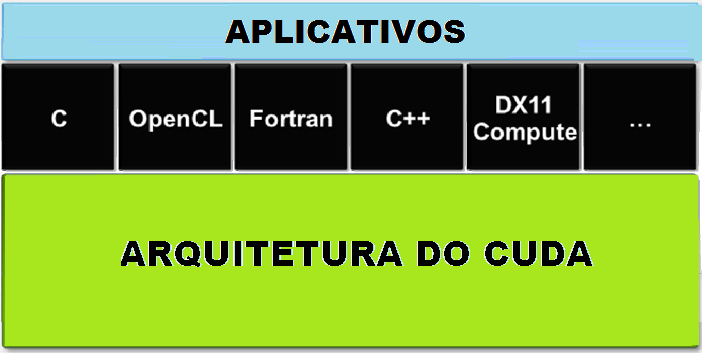
\includegraphics[scale=0.6]{LingSuportadas.eps}
	\caption{Linguagens Suportadas(adaptado de[\cite{cuda}])}
	\label{fig:lingsuportadas}
	\end{center}
\end{figure}

A arquitetura NVIDIA CUDA se baseia tanto em componentes de hardware como de software~[\cite{cuda}]. A parte que entendemos por software é a executada na CPU, formada por um algoritmo seqüencial escrito comumente na linguagem C ou alguma outra que é suportada por CUDA. A parte do hardware é formada pelo código compilado por CUDA para torná-lo um kernel. \textit{Kernel} são blocos que especificam parte do algoritmo em que se deseja a
paralelização. Ele também pode ser tratado como um código que pode ser utilizado pela GPU para chamar outros kernels nela ou em outra GPU.

A GPU contém milhares de threads. CUDA faz a formatação do código de uma maneira que threads sejam alocadas paralelamente e o usuário usufrua dessa característica, podendo fazer chamadas de kernel que serão independentes entre si, o que permite a GPU rodar vários algoritmos.

Podemos ver na figura \ref{fig:graficoscuda1} a diferença de potencial que uma GPU, com seu paralelismo, possui em relação a um processador (CPU):

\begin{figure}[!htb]
	\begin{center}
	\centering
			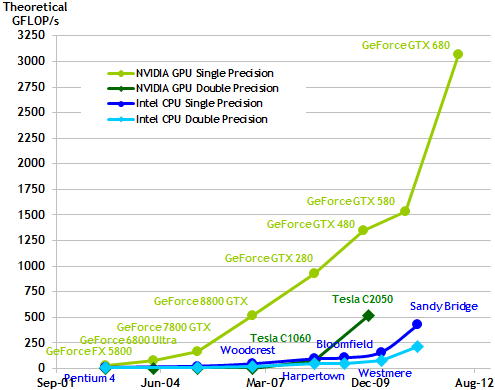
\includegraphics[scale=0.8]{ImageSub.eps}
	\caption{Operações de Ponto Flutuante por segundo para CPU e GPU(adaptado de [\cite{cuda}])}
	\label{fig:graficoscuda1}
	\end{center}
\end{figure}

Na figura \ref{fig:graficoscuda1} gráfico temos informações sobre o pico de operações por ponto flutuante. A GPU alcança a casa de TFlops/s, e a CPU apresenta um desempenho baixo mesmo comparado a arquiteturas de GPUs anteriores que não são compatíveis com CUDA.

\begin{figure}[!htb]
	\begin{center}
	\centering
			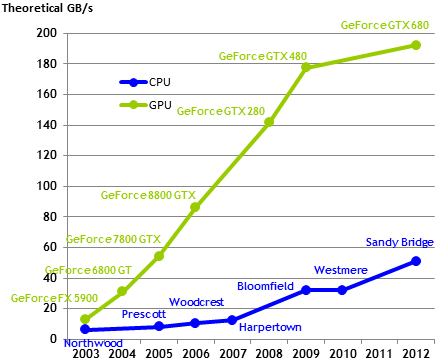
\includegraphics[scale=0.8]{ImageSub2.png}
	\caption{Tamanho de banda de memória para CPU e GPU(adaptado de [\cite{cuda}])}
	\label{fig:graficoscuda2}
	\end{center}
\end{figure}

A GPU é voltada para computação intensiva, com alta paralelização, que são características do problema de renderização gráfica. Além disso, sua arquitetura é especializada no processamento deste tipo de dados e não no controle de fluxo. Podemos visualizar essa diferença quando observamos a figura \ref{fig:transistores}.

\begin{figure}[!htb]
	\begin{center}
	\centering
			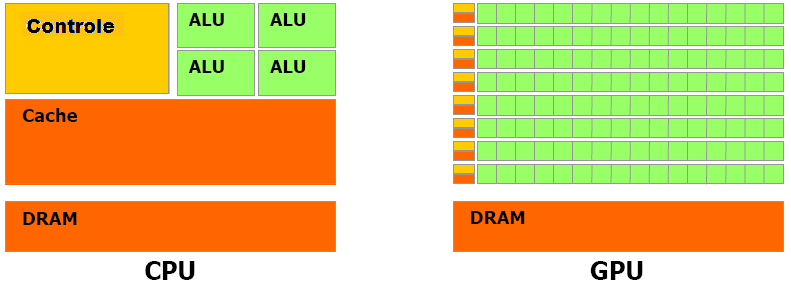
\includegraphics[scale=0.6]{transistores.eps}
	\caption{Quantidade de transistores para processamento de dados(adaptado de [\cite{cuda}])}
	\label{fig:transistores}
	\end{center}
\end{figure}

A quantidade de transistores utilizados para fazer processamento (ALU - \textit{Arithmetic Logic Unit}) é bem maior na GPU que na CPU. A arquitetura da CPU ainda está dividida em enormes blocos que contêm um componente de controle de fluxo e um de memória cache. No caso da GPU, o mesmo programa é executado em muitos elementos em paralelo. Dessa maneira, não possui um sofisticado componente de controle de fluxo, porém, oferece uma grande intensidade de computação aritmética. Além disso, a cache se torna pequena na GPU diminuindo a latência para execução de cada grande bloco de ALU's, diferente da CPU que contém uma cache enorme, obtendo uma latência alta para acesso. Possuindo uma unidade de controle, um componente de cache e um conjunto enorme de ALU's, é possível obter a estrutura de vários grupos de
cores. Podemos assim certificar que a GPU é um manycore, apresentando de 32 até 128 cores dependendo do modelo. Essa subdivisão de cores na GPU é chamada de \textit{Stream Processing}.

Um ponto importante a ser lembrado é que, para a execução na GPU, o algoritmo paralelizado não pode ter muita dependência de dados em cada passo de computação, pois a GPU não faz paralelização de tarefas e sim de processamento de dados. Caso essa otimização não seja feita no algoritmo, a GPU tem seu desempenho bastante afetado.

Com relação à hierarquia de compilação para o CUDA, a figura \ref{fig:pilhasoftware} ilustra a arquitetura da sua pilha de software.

\begin{figure}[!htb]
	\begin{center}
	\centering
			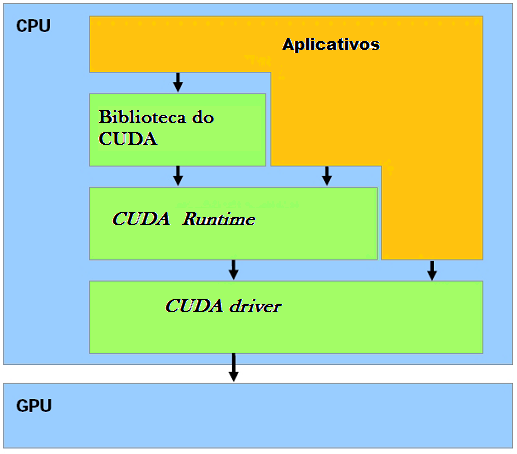
\includegraphics[scale=0.6]{pilhaSoftware.png}
	\caption{Pilha de Software(adaptado de [\cite{cuda}])}
	\label{fig:pilhasoftware}
	\end{center}
\end{figure}

Essa pilha de software mostra a hierarquia de execução de CUDA. A API de CUDA fornece suporte a diversas funções matemáticas, bibliotecas, suporte ao runtime e ao driver.

O CUDA \textit{runtime} ~[\cite{cuda}] é a camada de alto nível de programação, enquanto a camada do driver é a camada baixa para manipulação de dados. O CUDA driver gerencia e otimiza os recursos relacionados diretamente à GPU. CUDA é baseada em programação paralela, permitindo milhares de threads executando uma mesma tarefa. Neste caso, a GPU funciona como um co-processador da CPU, a qual chamamos de \textit{HOST} e a GPU de \textit{DEVICE}.

CUDA usa como base a linguagem C~[\cite{cuda}], que permite uma curva rápida de aprendizado. Nela deve-se criar funções desejadas que CUDA otimiza e paraleliza na GPU. Essas funções são chamadas de kernel. A seguir, observamos um exemplo de um código simples, em seguida, uma explanação sobre cada aspecto inerente ao entendimento seqüencial desse código.

%%%%%%%%COMENTAR COM O PROFESSOR ALGUMA SE A EXPLICAÇÃO ESTA BOA!!

\begin{verbatim}
__global__ void matAdd(float A[N][N], float B[N][N],
float C[N][N])
{
    int i = threadIdx.x;
    int j = threadIdx.y;
    C[i][j] = A[i][j] + B[i][j];
}


int main()
{
    // Kernel invocation
    dim3 dimBlock(N, N);
    matAdd<<<1, dimBlock>>>(A, B, C);
}

\end{verbatim}

Nesse código temos uma função matAdd que apresenta uma tag \textit{\_\_global\_\_} antes da definição da função. Essa tag define ao compilador que esse bloco será paralelizado na GPU.  Esta função recebe três matrizes de tamanho N por N, onde cada thread nos eixos x e y serão responsáveis por somarem as matrizes A e B, sendo atribuido o resultado da soma na matriz C.  Caso fosse desenvolvido um código similar no modo convencional, teria que aninhar dois laços de forma a percorrer todos os indices das matrizes. É claro, a diferença na forma de implementar e tratar o problema.

A função \textit{main} faz a invocação do método. Ele se localiza no HOST e o código é executado na GPU (DEVICE). Em um computador podemos encontrar mais que uma GPU, neste caso elas serão chamadas de DEVICE 0, DEVICE 1, etc. O kernel é acionado colocando uma \textit{tag} de configuração antes da declaração dos parâmetros, "$<<< >>>$". Há três parâmetros possíveis na configuração: a configuração do tamanho das \textit{grids} (A), a configuração do tamanho dos blocos (B) e a quantidade de memória compartilhada que se deseja utilizar no algoritmo (Ns). Isso gera uma configuração genérica "$<<<A,B,Ns >>>$".

No main, antes da invocação, declaramos um tipo de variável definida pelo CUDA chamada "dim3". A variável criada dimBlock terá três dimensões e cada uma dessas dimensões representará a dimensão de um bloco. No exemplo, teremos um bloco com tamanho $N$ para dimensão $x$, tamanho $N$ para dimensão $y$ e a dimensão $z$ que foi omitida tem tamanho 1. Desta forma, seguindo a lógica de desenvolvimento da aplicação é possível construir algoritmos paralelizados na GPU.


A arquitetura CUDA é baseada em \textit{arrays} escaláveis de multithreads SMs, ou thread Batching. Ele é um \textit{batch} de threads que o kernel executa e organiza em grids de threads block. Uma thread block é um batch de threads que cooperam entre si para compartilhar eficientemente as informações que serão processadas. Essa eficiência vai desde o compartilhamento (cópia da DRAM GPU para a memória compartilhada e vice-versa) dessa informação através da memória compartilhada, até a sincronização de execução para o acesso a essa memória.

Cada thread é identificada através de ID única, chamada thread ID. Há um número limitado de threads por bloco. Porém, um bloco de mesma dimensão e tamanho pode ser executado por um mesmo kernel fazendo um grid de blocos, aumentando ainda mais a quantidade de threads sendo executados em paralelo. Vale salientar que as threads de blocos diferentes não podem se comunicar.
Cada bloco é identificado por um block ID, e tem sua ID única em relação ao grid.

\begin{figure}[!htb]
	\begin{center}
	\centering
			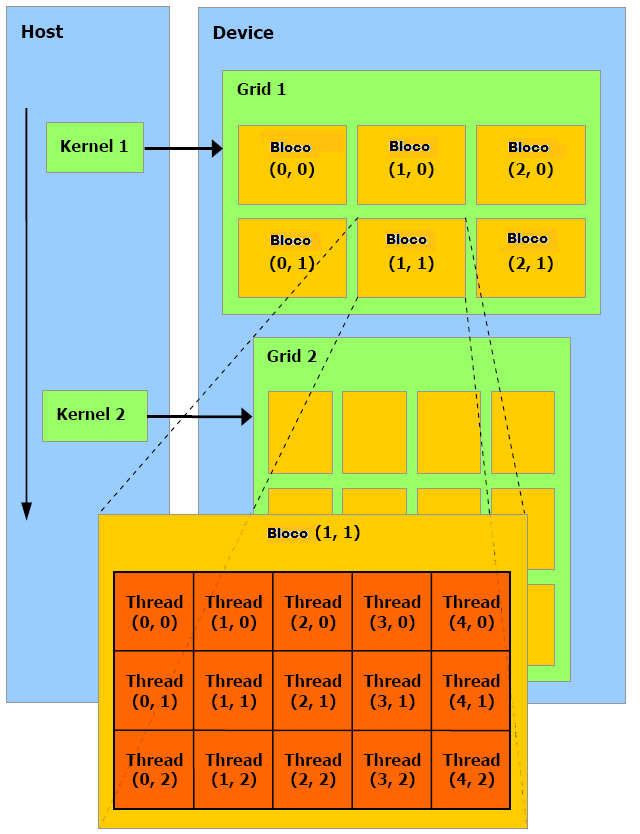
\includegraphics[scale=0.35]{ThreadBatching.eps}
	\caption{Batching de Threads(adaptado de [\cite{cuda}])}
	\label{fig:ThreadBatching}
	\end{center}
\end{figure}

Um multiprocessador é um nome formalizado para threads. Ele consiste de oito cores de processadores escalares, duas unidades de funções especiais transcendentais, uma unidade de controle de instruções multithread e uma memória compartilhada on-chip.

O multiprocessador cria, gerencia, e executa threads concorrentes com custo nulo de hardware no âmbito de gerenciamento de processos. Para gerenciar centenas de threads rodando em diferentes programas, o multiprocessador nas últimas versões de CUDA emprega o SIMT. O multiprocessador mapeia cada thread a um core de processador escalar, que executa independentemente suas próprias instruções e tem seu próprio estado de registradores.

Esse multiprocessador SIMT cria, gerencia, escalona e executa grupos de 32 threads paralelas chamadas de warps. Threads individuais que compõem o SIMT \textit{warp} podem começar sua execução juntas no mesmo programa, mas estão livres para ramificarem e executarem de forma autônoma. Contudo, se alguma thread ultrapassar a dependência condicional da ramificação, ela será desabilitada. 

A arquitetura SIMD(\textit{Single Instruction Multiple Data}) é implementada como um conjunto de múltiplos processadores que tem a capacidade de, com uma única instrução, em um mesmo ciclo de clock, processar várias informações.

\begin{figure}[!htb]
	\begin{center}
	\centering
			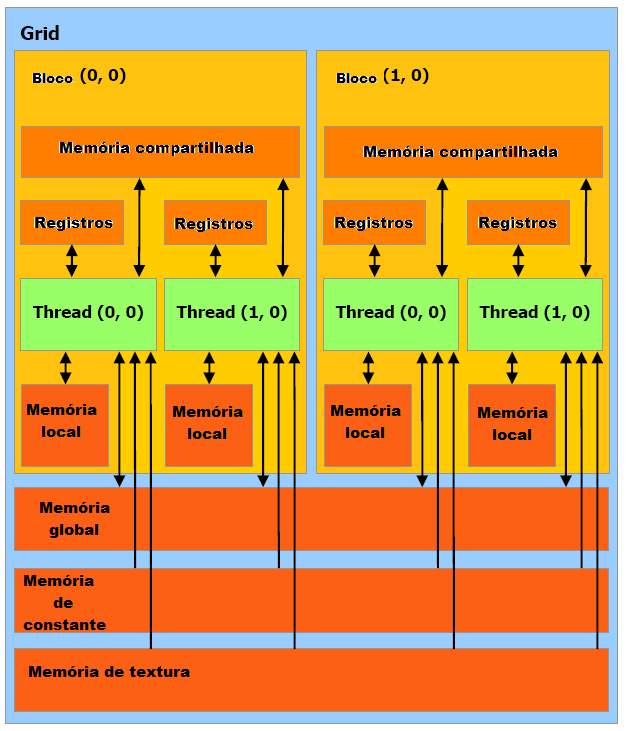
\includegraphics[scale=0.25]{HierarquiaMemoriasCuda.eps}
	\caption{Conjunto de Multiprocessadores e Hierarquia das Memórias(adaptado de [\cite{cuda}])}
	\label{fig: SIMT}
	\end{center}
\end{figure}

Como podemos observar cada multiprocessador possui: um conjunto de registradores de 32-bit, cache paralelo ou memória compartilhada que é partilhada com os outros processos, uma cache constante e outra de textura apenas para leitura. A memória local e global não é "cacheada" e pode ser escrita e lida pelos processos.
Um ponto forte de CUDA é que há uma separação na memória DRAM entre o HOST e o DEVICE. A API de CUDA fornece uma forma de transmissão de alta performance para transferir os dados entre esses dispositivos usando \textit{High Performance} (DMA), ou DMA de alto desempenho.

\section{Suporte ao Paralelismo de Tarefas}
Diversas ferramentas de programação suportam paralelismo de tarefas em CPUs mul- ticore. Recentemente, alguns trabalhos em andamento têm buscado oferecer suporte a esse paradigma também em sistemas híbridos compostos por CPUs e GPUs.



\subsection{StarPU}

O StarPU (AUGONNET et al., 2009) é uma ferramenta para programação paralela que oferece suporte para arquiteturas híbridas, como CPUs multicore e aceleradores. O StarPU propõe uma abordagem de tarefas independente da arquitetura base. São definidos codelets como uma abstração de uma tarefa que pode ser executada em um núcleo de uma CPU multicore ou submetido a um acelerador. Cada codelet pode ter múltiplas implementações, uma para cada arquitetura em que o codelet pode ser executado, utilizando as linguagens ou bibliotecas específicas para a arquitetura alvo. Uma aplicação StarPU é descrita como um conjunto de codelets com suas dependências de dados (AUGONNET; NAMYST, 2009).

A ferramenta possui um conjunto de políticas de escalonamento implementadas que o programador pode escolher de acordo com as características da aplicação. A principal delas faz uso do algoritmo de escalonamento estático HEFT (Heterogeneous Earliest Finish Time) para escalonar as tarefas com base em modelos de custo de execução das tarefas.

(...)

\subsection{Charm++}

No Charm++ as tarefas são representadas pelos chares, que são objetos paralelos e representam unidades locais de trabalho. Cada chare possui dados locais, métodos para tratamento de mensagens e possibilidade de criar novos chares, assim como processos MPI-2. Existe ainda um tipo especial de chare, chamado branch-office, que possui uma ramificação em cada processador e um único nome global. Branch- office chares oferecem métodos sequenciais que podem ser acessados por chares de forma transparente em qualquer processador.

No Charm++ a sincronização pode ser feita através de Futures, objetos de comunicação, replicados ou compartilhados. O future  é uma estrutura que serve para armazenar um valor que pode ser acessado no futuro por outro chare. O acesso a essa estrutura  é bloqueante e pode ser comparado a um acesso ao resultado de um m ́etodo spawned precedido de uma chamada sync. A utilização de objetos de comunicação permite que um chare se comunique por troca de mensagens, tornando a comunicação semelhante à realizada com MPI. Os demais objetos introduzem conceitos para comunicação n ̃ao encontrados nos outros ambientes.

O Charm (KALE et al., 1995) foi uma das primeiras implementaçõses do conceito de Atores, que são objetos concorrentes que se comunicam apenas por troca de mensagens. Charm++ (KALE; KRISHNAN, 1996) é baseado no Charm e suporta diferentes modos de compartilhamento de informações. Ele reúne recursos propostos em outros ambientes, como objetos sequenciais e paralelos, comunicação por troca de mensagens e futures. O Cilk (BLUMOFE et al., 1995)  é um ambiente de programacção paralelo focado em arquiteturas SMP. Ele  é baseado na linguagem C. O Cilk oferece também um escalonador de processos que é provado ser eficiente (VEE; HSU, 1999). Baseando-se no Cilk, foi desenvolvido um ambiente para execução de programas em arquiteturas com memória distribuída e aproveitamento de recursos ociosos, chamado Cilk-NOW (BLUMOFE; LISIECKI, 1997).

\subsection{Kaapi}

O XKaapi (INRIA; MOAIS; LIG, 2011) é uma reimplementação do KAAPI com suporte a paralelismo de tarefas "de grão fino". O KAAPI (GAUTIER; BESSERON; PI- GEON, 2007) (Kernel for Adaptative, Asynchronous Parallel and Interactive programming) é uma ferramenta para computação paralela em CPUs multicore e clusters. A implementação atual do XKaapi oferece suporte a arquiteturas multicore e extensões para suporte eficiente à GPUs foram propostas em (HERMANN et al., 2010; LIMA et al., 2012). O XKaapi é composto por um conjunto de APIs (Application Programming Interfaces) e pelo kernel, um ambiente de execução para as APIs que oferece escalonamento baseado em roubo de tarefas. A Kaapi++ é a interface do XKaapi baseada em um DFG (Data Flow Graph) para C++ e é dividida em três componentes: a assinatura da tarefa (task signature) onde são definidos o número e as características dos parâmetros da tarefa; a implementação da tarefa (task implementation) que especifica a implementação da tarefa para uma arquitetura e a criação da tarefa (task creation) que submete a tarefa para a pilha de execução.

\subsection{Cilk}

A ferramenta para programação paralela Cilk (BLUMOFE et al., 1995; FRIGO; LEI- SERSON; RANDALL, 1998; GROUP, 2012) é uma extensão da linguagem C para permitir a submissão, execução e sincronização de tarefas paralelas. A implementação de Cilk é baseada no algoritmo de escalonamento dinâmico por meio de roubo de tarefas apresentado em (BLUMOFE; LEISERSON, 1994). Cilk define tarefas como funções individuais que podem submeter novas tarefas dinamicamente. A sincronização é feita permitindo que as tarefas esperem pelas tarefas filhas, ou seja, tarefas que foram submetidas pela tarefa original.


\subsection{Intel TBB}

O Intel TBB (Threading Building Blocks) (REINDERS, 2010; CORPORATION, 2012) é uma biblioteca baseada em templates para programação paralela em C++ que faz uso de threads. Essa biblioteca permite expressar o paralelismo em diversos paradigmas de programação paralela como o paralelismo de dados, de laços ou de tarefas. As unidades de trabalho paralelas resultantes são escalonadas em threads por meio de um algoritmo de roubo de tarefas inspirado no ambiente Cilk.

\subsection{OpenMP}

OpenMP (Open Multi-Processing) (CHAPMAN; JOST; PAS, 2007) é uma ferramenta para programação paralela baseada na adição de diretivas de compilação em códigos C, C++ e Fortran. As diretivas OpenMP são utilizadas para indicar a paralelização de laços ou trechos de código. A partir da versão 3.0 (OpenMP ARB, 2008) foi inserido o conceito de tarefas, o que permite a utilização do paralelismo de tarefas através do uso de diretivas para delimitação de trechos de código como unidades de trabalho paralelas (AYGUADE et al., 2009). A especificação OpenMP (OpenMP ARB, 2008) não define uma política para o escalonamento das tarefas, ficando essa escolha a cargo de cada implementação.
	% Capítulo 1: Introdução
%\pagestyle{empty}
\cleardoublepage
\pagestyle{fancy}

\chapter{Algoritmo Proposto}\label{cap3}

\section{Introdução}\label{cap3:intro}

Esta seção demonstra detalhes de implementação do algoritmo proposto para o balanceamento de carga dinâmico em aglomerados de GPUs.


\section{Algoritmo}
Visão geral. O algoritmo proposto determina o tamanho do bloco ideal por processador usando uma abordagem de rebalanceamentos. Inicialmente, são encontradas as velocidades relativas de cada processador. Com esses valores são feitas curvas com um certo número de pontos e a partir dessas curvas geram-se modelos de execução de cada processador. O intuito é realizar uma regreessão sobre esses pontos e gerar uma curva que nos permite determinar o comportamento do modelo para cada processador. Processa-se uma quantidade relativamente pequena de dados, cujo limite superior é definido como uma percentagem fixa do total de dados, para a obtenção desses pontos. Começa-se com os maiores blocos possíveis para otimizar o tempo de execução, reduzindo o tamanho dos blocos com o passar dos rebalanceamentos. O tamanho do bloco diminui progressivamente à medida que a computação trabalha no sentido final para que todas as unidades de execução completem quase ao mesmo tempo. O algoritmo se resume a duas fases: uma fase chamada fase de adaptação e outra fase chamada fase de conclusão. O objetivo da primeira fase é determinar um peso a cada processador, que é utilizado na fase de conclusão do algoritmo.

Os pesos são calculados com base no tempo total necessário para a transferência de dados e o tempo de execução. Isto é essencial para o balancemanto de carga preciso.

Fase de adaptação: Esta fase encontra a velocidade relativa das unidades de computação que resultam em pesos para serem usado na fase de conclusão. O principal desafio é a de manter a fase inicial de adaptação o mais curta possível de modo a que a maior parte dos dados seja deixada para a fase de conclusão. 

Para conseguir isso, começa-se com tamanhos de blocos pequenos inicialmente e aumentá-os gradualmente com base no desempenho observado até que seja possivel determinar o cálculo preciso para os pesos para cada dispositivo.

A fase de adaptação primeiro mede o número de iterações concluídas na etapa anterior por unidade de tempo. Isto fornece o peso computacional, uma velocidade relativa de processamento para o último passo . Se a mudança de pesos entre o passo anterior e etapa atual é inferior a MIN altera-se a taxa ( que é definido como 0,01, o qual é considerado estável). Caso contrário, é preciso aumentar o tamanho do bloco para a próxima etapa.

A fim de alcançar a convergência dos pesos, estima-se uma curva para cada processador usando o método de Gauss-Newton. Uma vez que os parâmetros são obtidos, estima-se um peso computacional estável para cada processador e assim um tamanho estimado do bloco para cada processador.

Depois que o tamanho estimado do bloco é enviado para o processador, na solicitação de bloco seguinte, o algoritmo verifica se a estimativa é precisa, calculando o peso computacional novamente. Se a mudança de peso ainda não é estável, o processo de estimativa continua.

Uma vez que um peso computacional é  estável, o algoritmo continua aumentando tamanhos de bloco para outros processadores instáveis ​​até que todos os pesos se tornem estáveis ou uma percentagem fixa (20\%) de todos os dados serem processados. O último caso é um limite superior forçado para limitar a duração da fase de adaptação .

Fase de conclusão. Uma vez que todos os pesos são estáveis​​, o algoritmo passa para a fase de conclusão. Tamanhos de blocos da fase de adaptação não são mais usados. Em vez disso, o algoritmo usa o Guided Self-Scheduling modificado (MGSS) para encontrar o tamanho dos blocos corretos. A fase de conclusão integra pesos computacionais calculados na etapa anterior em MGSS. Eq. \ref{eq: gss} é a fórmula original GSS, que simplesmente divide o restante número de iterações de R para o número total de processadores P. MGSS utiliza Eq. \ref{eq: mgss} que distribui a R processadores proporcional ao seu peso $w_i$ calculado.

\begin{equation}
 	B = R/P
\end{equation}

\begin{equation}
 	B = R w_i/ \sum_{j=1}ˆ{P} w_j
\end{equation}

MGSS é mais adequado com a computação heterogênea porque ele começa com o maior tamanho de bloco possível e aceleradores são melhor utilizados com tamanhos de blocos maiores. Com os pesos computacionais estimado com precisão, a prova para o GSS original é válida para o MGSS. Isto é devido ao fato de os tamanhos de bloco diferentes calculados para diferentes processadores para o mesmo número de iterações restante terá sempre a mesma quantidade de tempo, porque pesos computacionais causam distribuição proporcional de blocos. 

\section{Implementação}
A implementação foi feita no arcabouço StarPU na linguagem C. Para cada dispositivo foi programado um codelet, com as caractereisticas dos dispositivos. A codelet é uma estrutura que representa uma função computaciona;. Cada codelet pode conter uma implementação do mesmo kernel em diferente arquiteturas (exemplo, CUDA, x86). 

\section{Resultados}

\subsection{Multiplicação de Matrizes}

A figura \ref{fig:1maquina} apresenta o algoritmo executando em uma única máquina. Neste caso o problema tratado é o de multiplicação de matrizes, com complexidade  $O(nˆ2)$. Nota-se que no caso do algoritmo proposto chamado de dinâmico e o HDSS, praticamente não há diferenças significativas na execução.

\begin{figure}[htb]
	\begin{center}
	\centering
			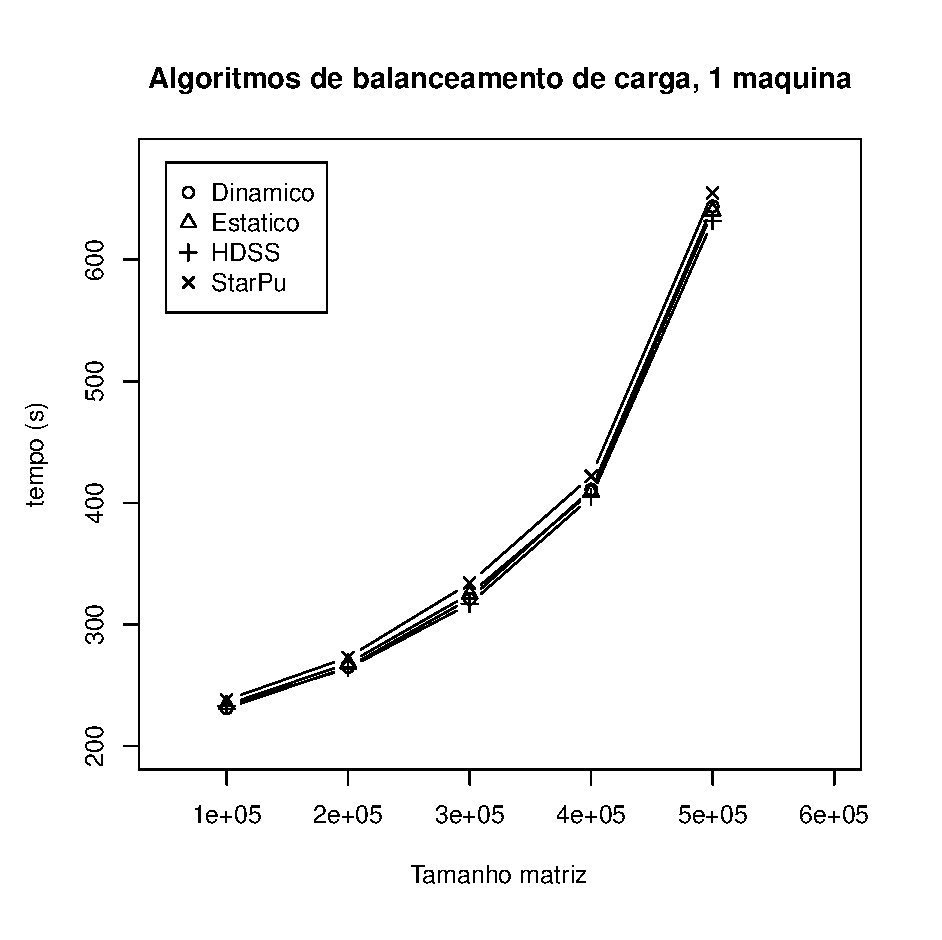
\includegraphics[scale=0.6]{1maquina.eps}
	\caption{Execução do algoritmo em uma máquina}
	\label{fig:1maquina}
	\end{center}
\end{figure}

A figura \ref{fig:2maquina} apresenta o algoritmo executando em duas máquinas.  Neste caso o algoritmo dinâmico leva uma leve vantagem em relação ao HDSS, mas ainda não siginificativa.

\begin{figure}[htb]
	\begin{center}
	\centering
			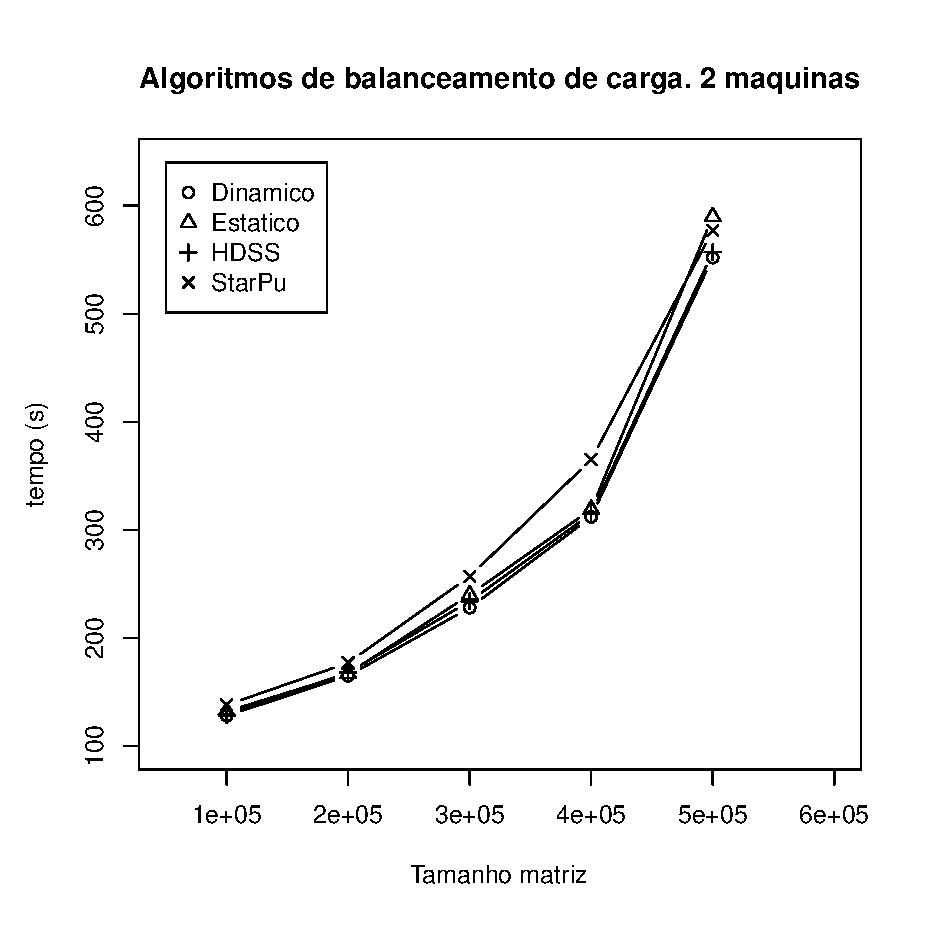
\includegraphics[scale=0.6]{2maquinas.eps}
	\caption{Execução do algoritmo em duas máquinas)}
	\label{fig:2maquina}
	\end{center}
\end{figure}


A figura \ref{fig:3maquina} apresenta o algoritmo executando em três máquinas.  No último caso, oo dinâmico apresentou uma vantagem maior em relação ao HDSS, o que nos revela uma vantagem mais relevante em meios mais hetererogêneos. 

\begin{figure}[htb]
	\begin{center}
	\centering
			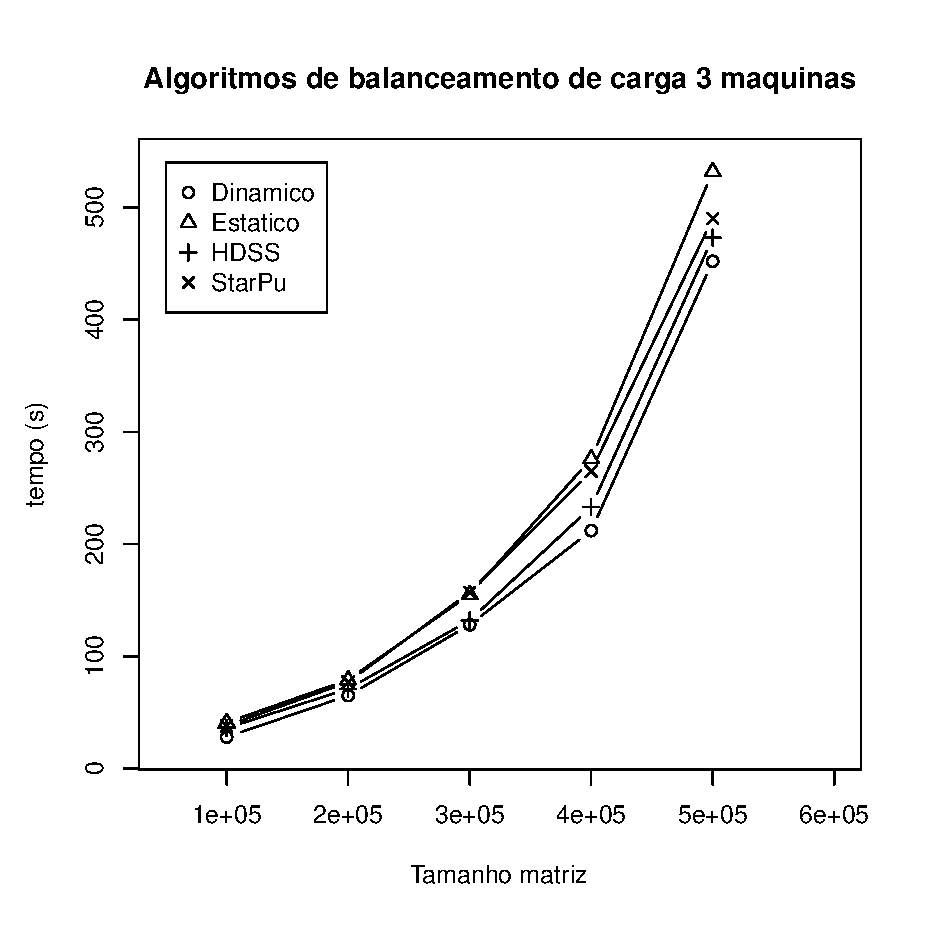
\includegraphics[scale=0.6]{3maquinas.eps}
	\caption{Execução do algoritmo em três máquinas)}
	\label{fig:3maquina}
	\end{center}
\end{figure}

A razão da maior adaptabilidade do algorimto perante os outros algortimos é devido ao método de Newton utilizado nos rebalanceamentos, no faz com que em meios heterogêneos a resolução do sistema de equações seja feita de forma mais eficiente, em relação por exemplo o HDSS, que realiza uma distribuição uniforme da carga na fase de conclusão.



\begin{figure}[htb]
	\begin{center}
	\centering
			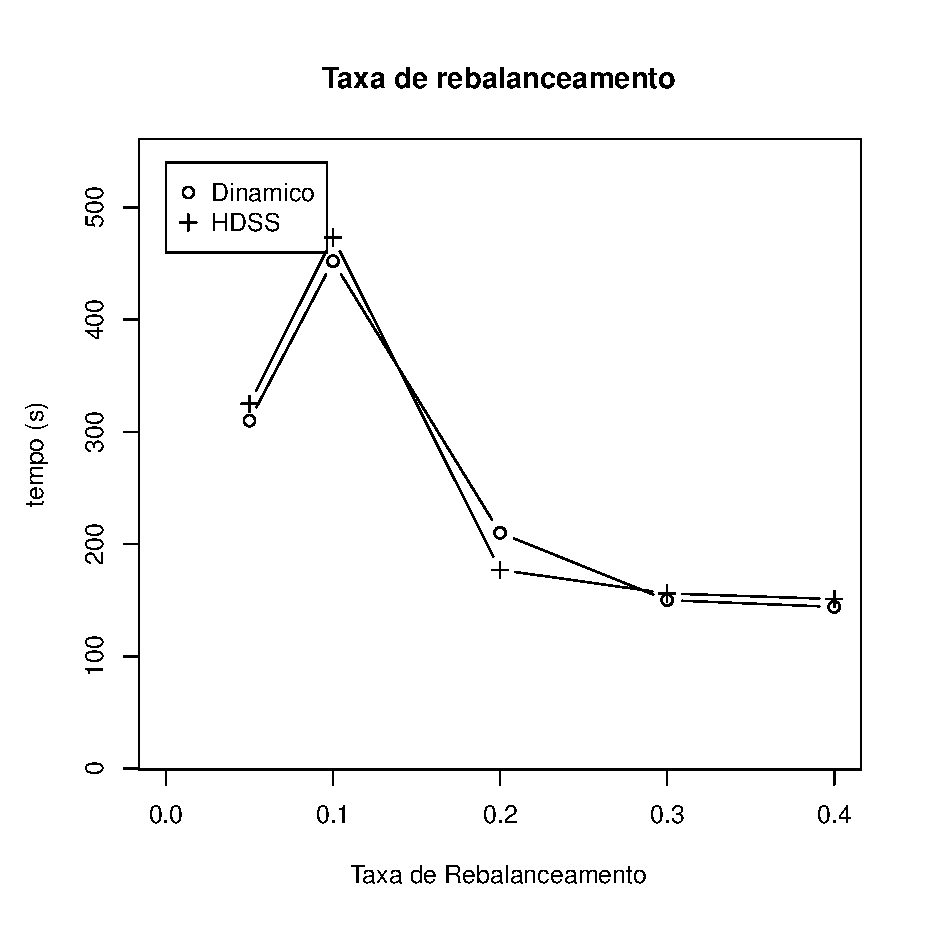
\includegraphics[scale=0.6]{TaxaRebalancemento.eps}
	\caption{Execução do algoritmo em três máquinas, alterando a taxa de rebalancemanto)}
	\label{fig:rebalanceamento}
	\end{center}
\end{figure}

Na figura \ref{fig:rebalanceamento} é variada a taxa de rebalancemento, o que influiencia a quantidade de vezes que é feito o rebalanceamento. Se a quantidade de rebalancemento for elevada o algoritmo faz varios rebalancemantos desnecessários, se baixa a distribuicão de carga não ocorre, o que torna o algoritmo estático. Percebe-se pela figura que o melhor valor para um dado tamanho de matriz é  o de 0.1. Neste caso o numero de rebalancementos encontra-se não elevado, mas ocorre durante a fase de conclusão.


\section{IPOPT}

IPOPT (Interior Point Optimizer) é um pacote de software aberto para otimização não linear. IPOPT pode resolver problemas de programação não-linear da seguinte forma:
	
\begin{equation}
 	min f(x)

	sujeito a: g^L < g(x) < g^U \\
			x^L< x < x^U
\end{equation}

onde x $\in$ a $\Re ^ n$ são as variaveis de otimização, $f : R^n em R$ é a função objetivo, e $g: R^n em R^M$ são as restrições não lineares. A função f(x) e g(x) podem ser linear ou não linear.  

Para resolver um problema de otimização precisa-se criar um IpoptProblem com a função CreateIpoptProblem, que posteriormente precisa ser passado para a função IpoptSolve. O IpoptProblem criado por CreateIpoptProblem contem as dimensões do problema, as variaveis e os limites das restrições.







	% Capítulo 2: ... Experimentos
%\include{cap3} % Capitulo 4: Explicação da Implementação da MLP e resultados preliminares
%\pagestyle{empty}
%\cleardoublepage
\pagestyle{fancy}
\chapter{Balanceamento de Carga}

\section{Balanceamento de Carga}\label{cap2:mem}

Capitulo dedicado a explicação dos principais algoritmos de balanceamento de carga, realcionando com o nosso trabalho.	% Capítulo 3: Considerações Finais

% Formato da bibliografia
\bibliographystyle{apalike}
% Arquivo .bib
\bibliography{bibQualificacacao}

% Apêndice(s)
%\include{apendice}

% Fim do texto
\end{document}
